\section{Nombre: Ciudadanos} \label{per:ciudadanos}  
\subsection{Descripción:}
Personas comunes de la época prehispánica mesoamericana.
\begin{itemize}
	\item \textbf{Hombre con jarrón:}
	Esclavo de mediana  edad. Viste un taparrabos de manta blanca. Sobre su espalda carga un jarrón de gran tamaño, sus manos se encuentran entrelazadas por detrás de su espalda para servir como soporte al jarrón. Lleva el cabello atado en una media cola, el cabello le llega a la altura de los hombros. Va descalzo.
	\item \textbf{Hombre con cacao:}
	Esclavo de mediana edad. Viste un taparrabos de manta blanca. Sobre su espalda carga seis sacos de cacao apilados unos sobre otros, sus manos se encuentran entrelazadas por detrás de su espalda para servir como soporte, su espalda se muestra inclinada a manera de mostrar que lo que carga es pesado. Lleva el cabello atado en una media cola, el cabello le llega a la altura de los hombros. Va descalzo.	
\item \textbf{Hombre noble:}
	Noble de mediana edad. Viste una capa roja cruzada de lado derecho por lo que su brazo izquierdo queda libre. La capa le llega a la altura de la entrepierna. Además de la capa porta un taparrabos de manta blanco. Lleva el cabello atado en una media cola, el cabello le llega a la altura de los hombros. Dado que se encuentra en una ciudad no tan importante para el imperio y no ostenta un rango tan alto dentro de la nobleza va descalzo.
	\item \textbf{Mujer con jarrón:}
	Ciudadana de mediana edad. Viste una falda larga a la altura de los tobillos y una blusa de cuello rectangular, ambas prendas de manta blanca. Sobre su cabeza carga un jarrón de gran tamaño. Lleva el cabello arreglado en un chongo. No usa zapatos.
	\item \textbf{Mujer de puesto:}
	Comerciante de mediana edad. Lleva el cabello recogido en un chongo. Viste un huipil blanco. Se muestra sentada sobre  un tapete y frente a ella hay artesanías de color blanco: dos vasos y un tazón.	
	\end{itemize} 
\subsection{Status:}
\begin{itemize}
		\item Personaje no jugable.
	\end{itemize}
\subsection{Imagen}
Ver figura \ref{fig:Ciudadanos}.
\begin{figure}
	\centering
	\subfigure[Hombre con jarrón.]{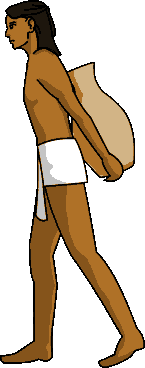
\includegraphics[scale=0.5]{Imagenes/hombre02}}
	\subfigure[Hombre con cacao.]{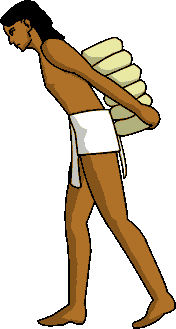
\includegraphics[scale=0.5]{Imagenes/hombre01}}
	\subfigure[Hombre noble.]{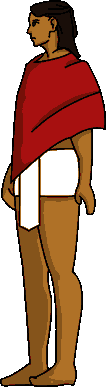
\includegraphics[scale=0.5]{Imagenes/hombre03}}
	\subfigure[Mujer con jarrón.]{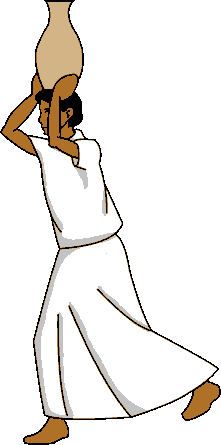
\includegraphics[scale=0.5]{Imagenes/mujer01}}
	\subfigure[Mujer de puesto.]{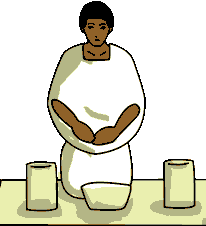
\includegraphics[scale=0.5]{Imagenes/mujer02}}
	\caption{Ciudadanos que se encuentran.}
	\label{fig:Ciudadanos}
\end{figure} 
\subsection{Concepto:}
Los ciudadanos se encuentran para relatar al jugador la época en la que se encuentra, la situación actual que enfrentan, el lugar donde se encuentran y más datos para entender el contexto que lo rodea.
\subsection{Encuentro:}
En el nivel 1.
\subsection{Bloques de animación:}
	\begin{itemize}
		\item Mujer comerciante. 
			\begin{itemize}
				\item Animación mover mercancía de un lado a otro.
			\end{itemize}
		\item Mujer jarrón.
			\begin{itemize}
				\item Animación caminar.
			\end{itemize}			 
		\item Hombre jarrón.
			\begin{itemize}
				\item Animación caminar.
			\end{itemize} 
		\item Hombre cacao.
			\begin{itemize}
				\item Animación caminar.
			\end{itemize}
		\item Hombre noble.
			\begin{itemize}
				\item Animación revisar mercancía(Si esta cerca de un puesto). 
				\item Animación platicar (Si esta cerca de otro noble).
				\item Animación contar granos de cacao (Si no esta cerca de un puesto o de un noble).
			\end{itemize}				
	\end{itemize}	